\chapter{ParaView}
\label{chap:paraview}

This chapter provides a brief introduction to several basic ParaView workflows
used to inspect Dendro simulation output. We begin by loading simulation files,
then describe how to create slices, visualize fields, use the Calculator filter,
adjust color maps, export data, and locate regions of interest.

\section{Opening Simulation Data}
\label{sec:paraview-opening-data}

To load data into ParaView, click the \textbf{Open File} button in the top-left
toolbar. This button is highlighted in Fig.~\ref{fig:paraview-open}.

\begin{figure}[h!]
\centering

\begin{tikzpicture}
% Image
\node[anchor=south west, inner sep=0] (img) at (0,0)
{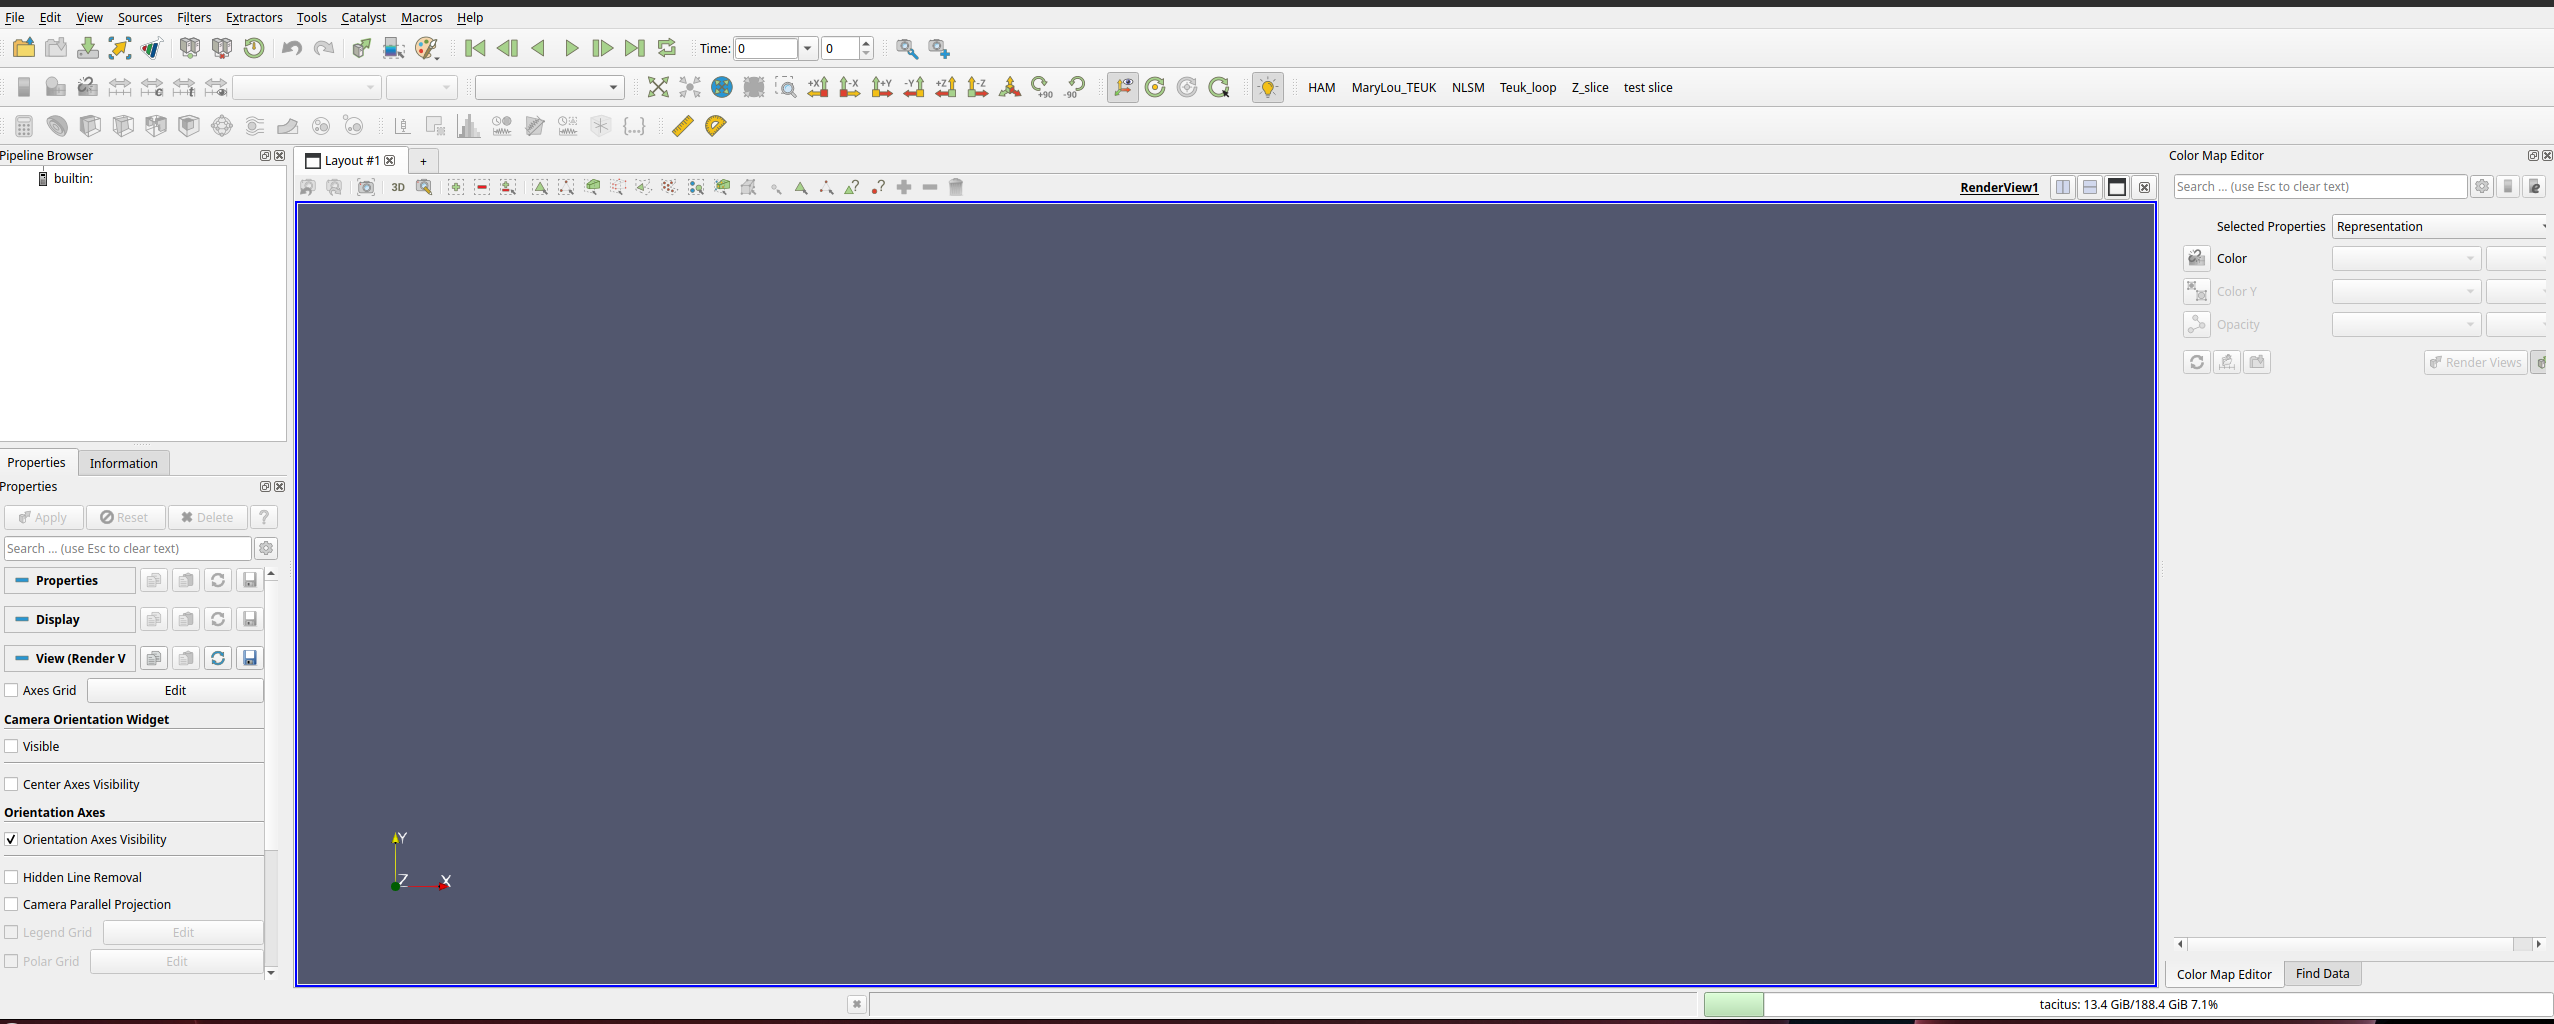
\includegraphics[width=\textwidth]{Paraview/Paraview_1.png}};

% Coordinates are scaled so that (0,0) is the bottom-left
% of the image and (1,1) is the top-right.
\begin{scope}[
    x={(img.south east)},
    y={(img.north west)}
]

    % Red box around the Open File icon
    \draw[red, very thick]
        (0.003,0.930) rectangle (0.018,0.968);

    % Arrow and label
    \draw[red, very thick, ->]
        (0.120,0.900) -- (0.018,0.955);

    \node[
        red,
        fill=white,
        draw=red,
        thick,
        rounded corners,
        font=\small
    ] at (0.180,0.890)
        {Open File};

\end{scope}

\end{tikzpicture}

\caption[Opening simulation data in ParaView]{
The ParaView interface with the \textbf{Open File} icon highlighted.
}
\label{fig:paraview_open}

\end{figure}

After clicking the \textbf{Open File} button, navigate to the directory where
the simulation output is saved. Dendro commonly writes visualization data in
\texttt{.vtu} format, which stands for \emph{VTK Unstructured Grid}. For
parallel runs, the output is often accompanied by a \texttt{.pvtu} file. The
\texttt{.pvtu} file acts as a wrapper that tells ParaView how the individual
\texttt{.vtu} pieces fit together.

In most cases, one should open the \texttt{.pvtu} file rather than opening the
individual \texttt{.vtu} files by hand. This allows ParaView to load the full
parallel dataset as a single object.

\section{Creating a Slice}
\label{sec:paraview-creating-slice}

Once the data has been loaded, a common operation is to create a two-dimensional
slice through the three-dimensional dataset. In this example, the
\textbf{Slice} tool is used to create a slice through the data, as shown in
Fig.~\ref{fig:paraview-slice-button}.

\begin{figure}[h!]
\centering

\begin{tikzpicture}
% Main screenshot
\node[anchor=south west, inner sep=0] (img) at (0,0)
{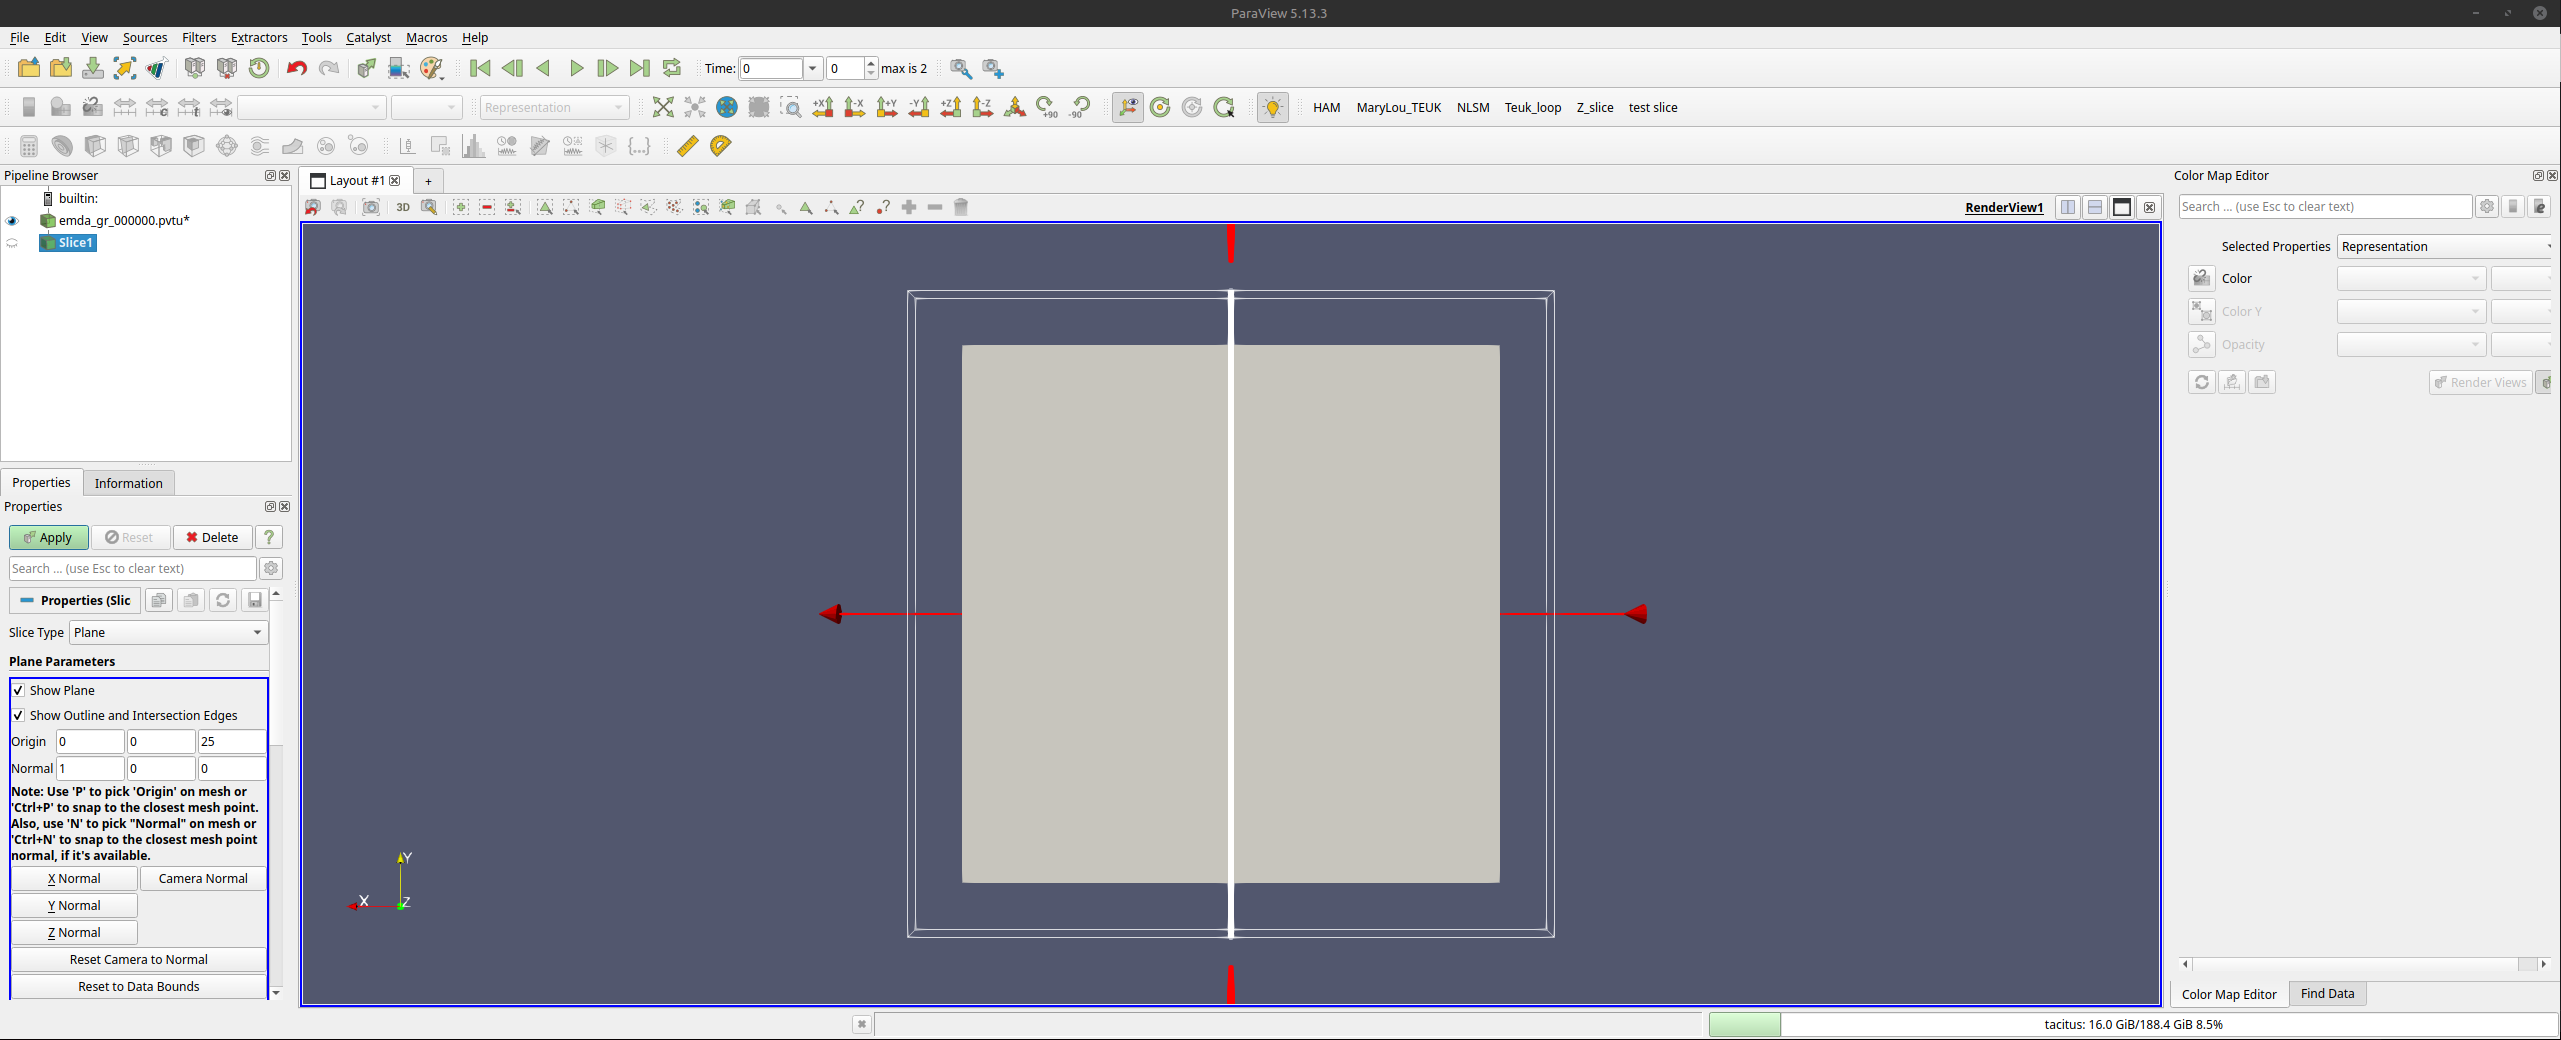
\includegraphics[width=\textwidth]{Paraview/Paraview_3.png}};

% Normalized image coordinates:
% (0,0) = bottom-left, (1,1) = top-right.
\begin{scope}[
x={(img.south east)},
y={(img.north west)}
]

```
% Box around the Slice toolbar button
\draw[red, very thick]
    (0.04415,0.847) rectangle (0.05842,0.877);

% Arrow and label for Slice
\draw[red, very thick, ->]
    (0.3215,0.70) -- (0.06,0.860);

\node[
    red,
    fill=white,
    draw=red,
    thick,
    rounded corners,
    font=\small
] at (0.33,0.69)
    {Slice};

% Box around the Calculator toolbar button
\draw[blue, very thick]
    (0.006,0.84) rectangle (0.018,0.88);

% Arrow and label for Calculator
\draw[blue, very thick, ->]
    (0.25,0.36) -- (0.018,0.840);

\node[
    blue,
    fill=white,
    draw=blue,
    thick,
    rounded corners,
    font=\small
] at (0.25,0.36)
    {Calculator};
```

\end{scope}

\end{tikzpicture}

\caption[ParaView Slice and Calculator tools]{
The ParaView interface with the \textbf{Slice} and \textbf{Calculator} tools
highlighted.
}
\label{fig:paraview_slice_button}

\end{figure}


After selecting the \textbf{Slice} tool, ParaView displays the slice settings
in the Properties panel. These settings determine the location and orientation
of the slicing plane.

\section{Adjusting the Slice and Viewing Data}
\label{sec:paraview-adjusting-slice}

ParaView allows the user to choose how the data should be sliced. Often, we want
to create $z$-slices, since this is the default orientation used for many
Dendro visualizations. To do this, set the slice normal to $(0,0,1)$. We also
set the origin to $(0,0,10^{-5})$. The small nonzero $z$-value is used because
setting the slice exactly at $z=0$ can sometimes cause ParaView to miss cells
lying on the symmetry plane.

The \textbf{Show Plane} option should be turned off so that only the data slice
is displayed. After changing these settings, click \textbf{Apply}.

Once the slice is displayed, the visualized field can be changed using the
field-selection menu. The available time steps can be explored using the time
controls, and the representation menu can be used to switch between viewing
modes such as \textbf{Surface} and \textbf{Wireframe}. These controls are
highlighted in Fig.~\ref{fig:paraview-view-controls}.

\begin{figure}[h!]
\centering

\begin{tikzpicture}
% Main screenshot
\node[anchor=south west, inner sep=0] (img) at (0,0)
{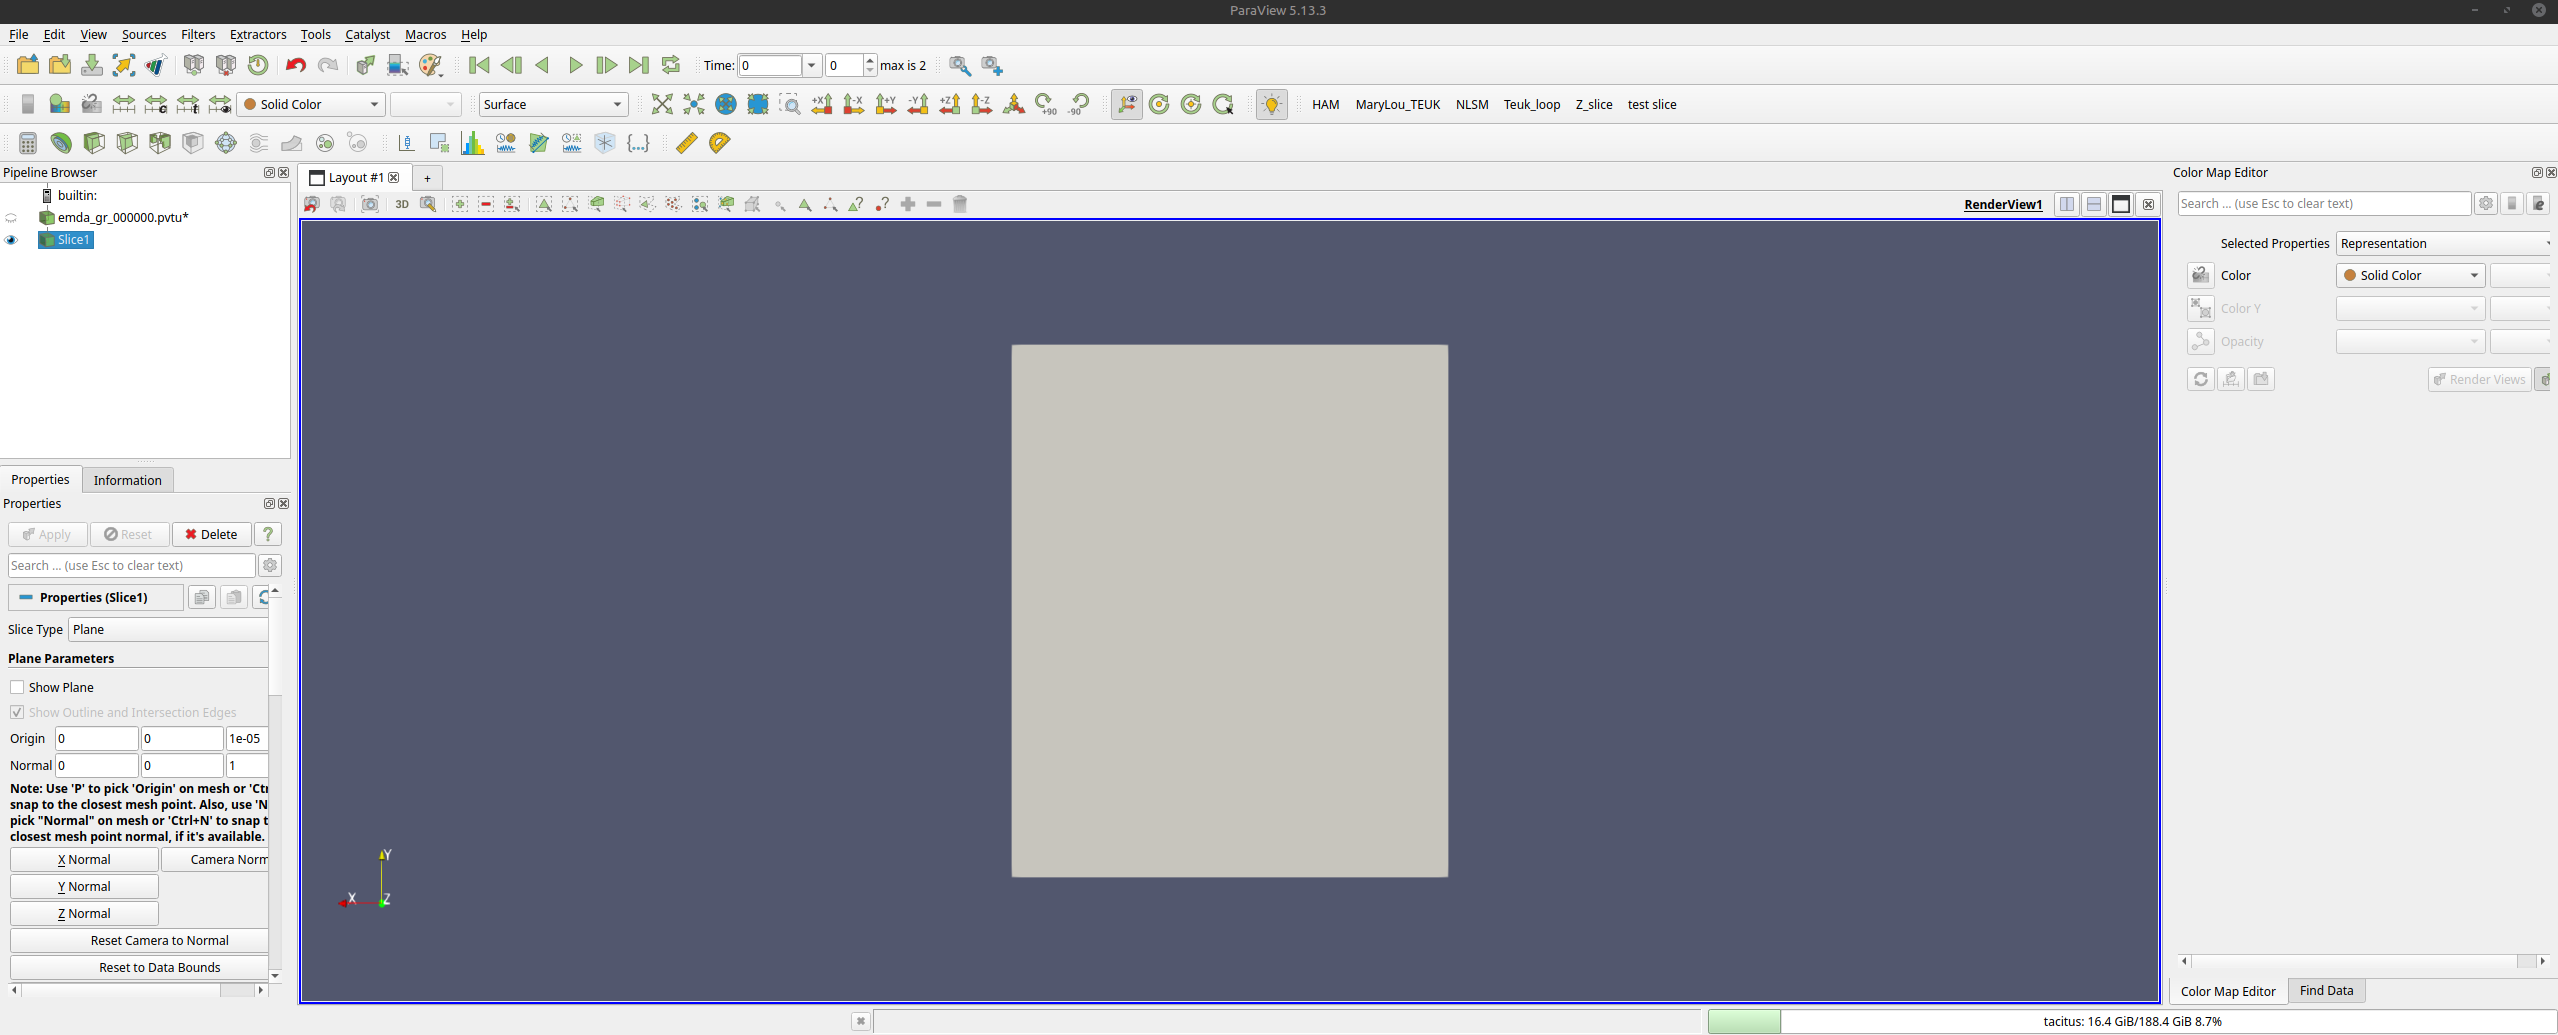
\includegraphics[width=\textwidth]{Paraview/Paraview_5.png}};

% Normalized image coordinates:
% (0,0) = bottom-left, (1,1) = top-right.
\begin{scope}[
x={(img.south east)},
y={(img.north west)}
]

```
% Time controls: play/pause and step forward/backward buttons
\draw[red, very thick]
    (0.18,0.921) rectangle (0.26,0.955);

\draw[red, very thick, ->]
    (0.330,0.975) -- (0.262,0.93);

\node[
    red,
    fill=white,
    draw=red,
    thick,
    rounded corners,
    font=\small
] at (0.385,0.975)
    {Time controls};

% Solid Color dropdown
\draw[blue, very thick]
    (0.087,0.885) rectangle (0.150,0.916);

\draw[blue, very thick, ->]
    (0.055,0.845) -- (0.118,0.883);

\node[
    blue,
    fill=white,
    draw=blue,
    thick,
    rounded corners,
    font=\small
] at (0.030,0.840)
    {Fields};

% Surface/Wireframe dropdown
\draw[green, very thick]
    (0.187,0.880) rectangle (0.245,0.916);

\draw[green, very thick, ->]
    (0.315,0.83) -- (0.246,0.890);

\node[
    green,
    fill=white,
    draw=green,
    thick,
    rounded corners,
    font=\small
] at (0.375,0.840)
    {Surface / Wireframe};
```

\end{scope}

\end{tikzpicture}

\caption[ParaView visualization and time controls]{
ParaView controls for stepping through time, selecting the displayed field or
color option, and switching between representations such as \textbf{Surface}
and \textbf{Wireframe}.
}
\label{fig:paraview_view_controls}

\end{figure}

\section{Using the Calculator}
\label{sec:paraview-calculator}

The \textbf{Calculator} filter can be used to construct derived quantities from
the fields stored in the simulation output. After selecting the loaded dataset
or slice, click the \textbf{Calculator} button. In the Calculator panel, choose
the appropriate scalar or vector fields from the available data arrays.
Mathematical operations can then be applied to these fields to define a new
quantity for visualization or export.

For example, the Calculator can be used to rescale a field, combine multiple
fields, or construct diagnostic quantities that are not stored directly in the
output files. After entering the desired expression, click \textbf{Apply} to
create the new field.

\section{Warping by Scalar}
\label{sec:paraview-warp-by-scalar}

The \textbf{Warp By Scalar} filter can be used to displace a surface according
to the value of a scalar field. This is useful for visualizing the relative
amplitude of a field on a slice.

To use the filter, click \textbf{Filters} and search for \textbf{Warp By
Scalar}. After selecting the filter, its settings appear in the Properties
panel, in the same general location as the slice settings.

\begin{figure}[h!]
\centering

\begin{tikzpicture}
\node[anchor=south west, inner sep=0] (img) at (0,0)
{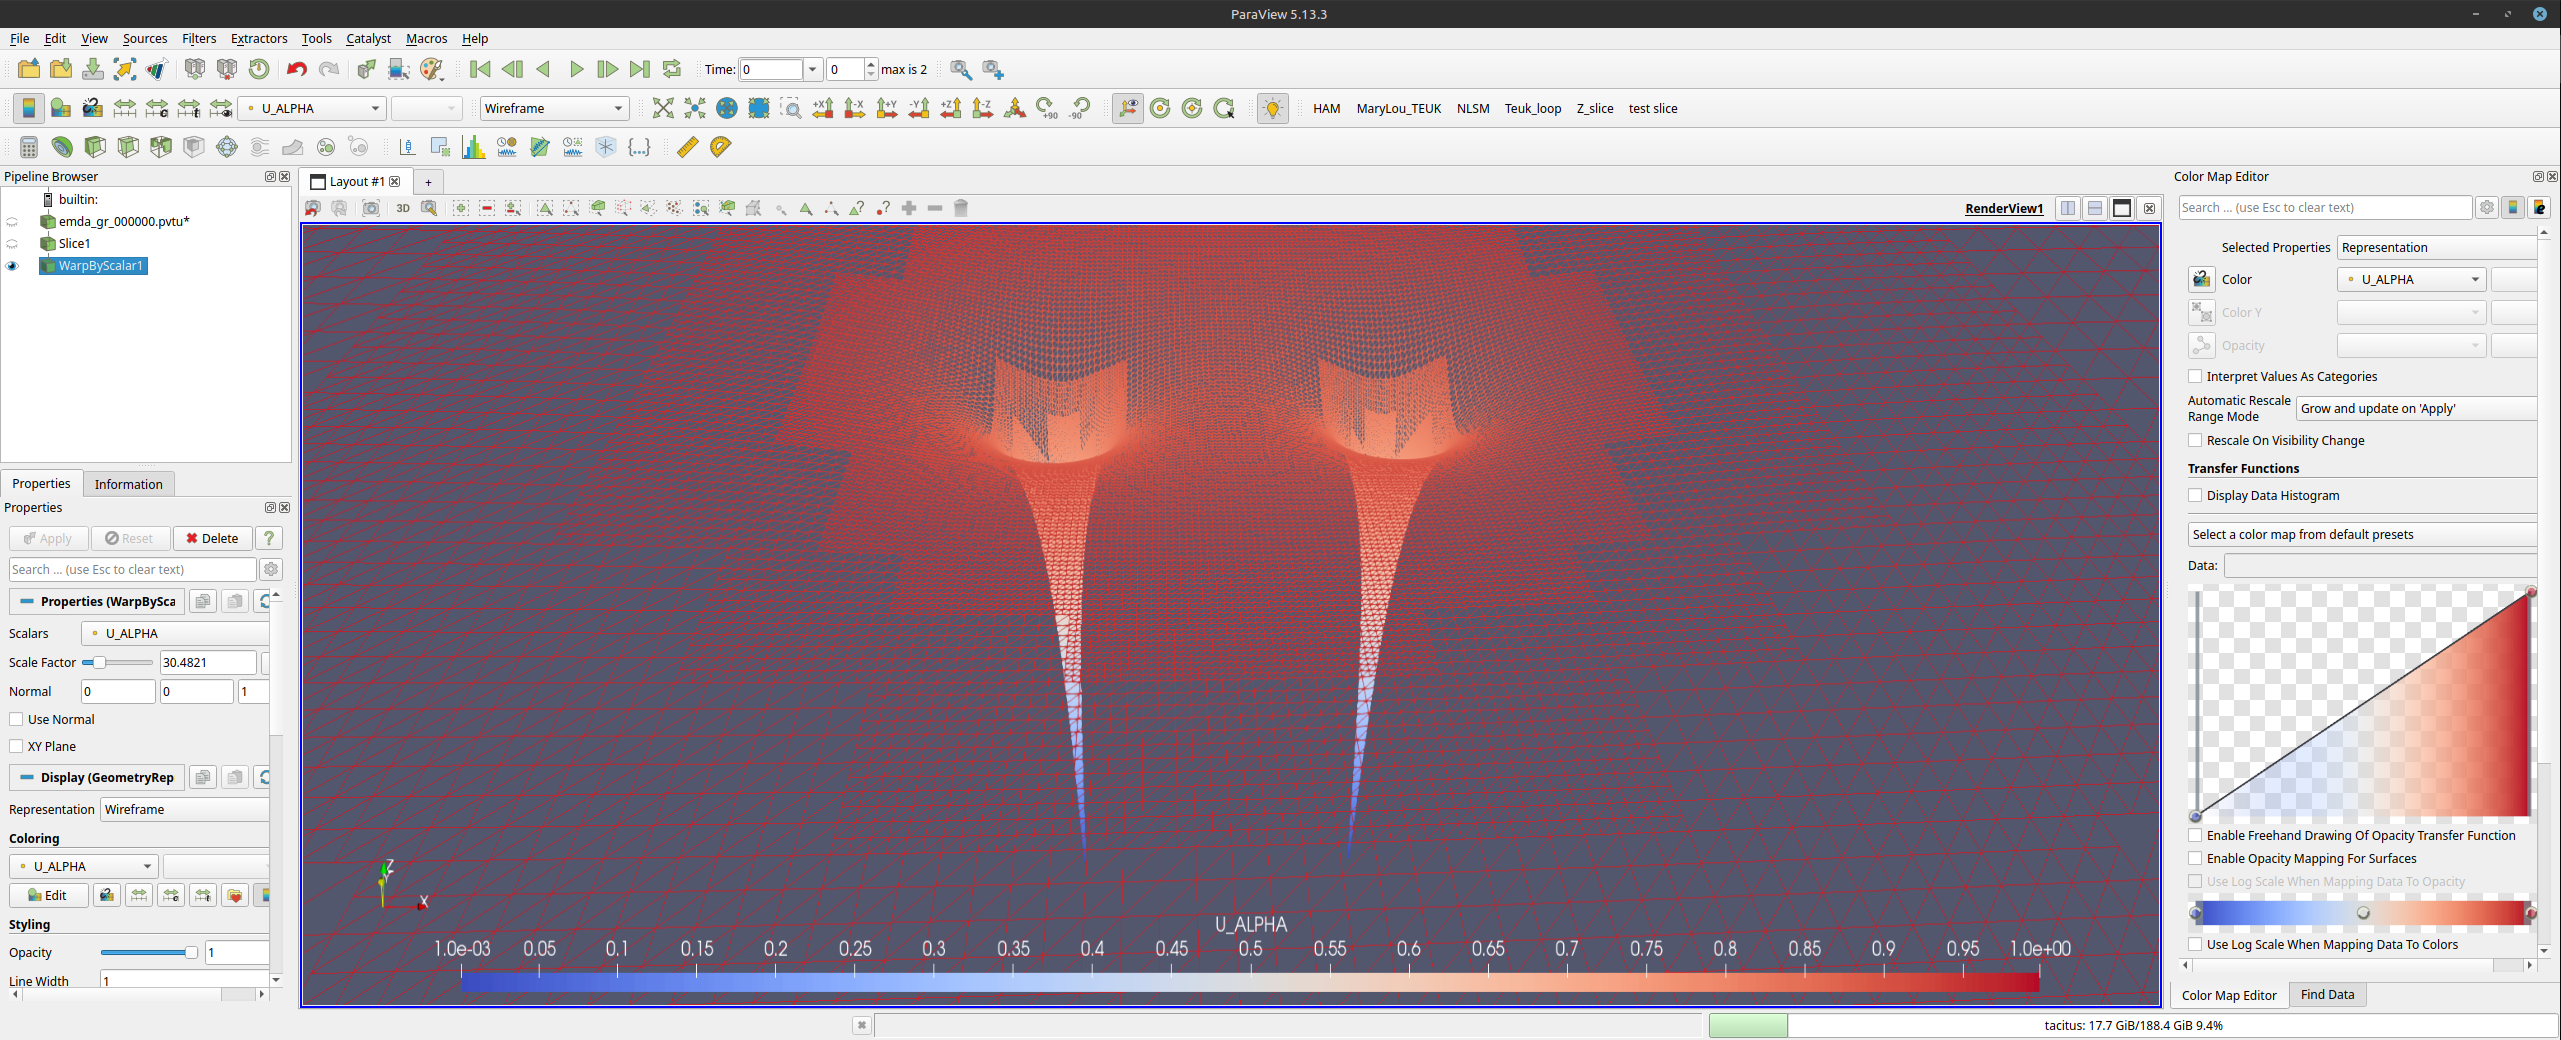
\includegraphics[width=\textwidth]{Paraview/Paraview_6.png}};

\begin{scope}[
x={(img.south east)},
y={(img.north west)}
]

```
% Scalars dropdown
\draw[red, very thick]
    (0.031,0.380) rectangle (0.084,0.410);

\draw[red, very thick, ->]
    (0.200,0.440) -- (0.085,0.410);

\node[
    red,
    fill=white,
    draw=red,
    thick,
    rounded corners,
    font=\small
] at (0.205,0.450)
    {Scalars};

% Scale Factor control
\draw[blue, very thick]
    (0.000,0.350) rectangle (0.100,0.381);

\draw[blue, very thick, ->]
    (0.165,0.360) -- (0.100,0.350);

\node[
    blue,
    fill=white,
    draw=blue,
    thick,
    rounded corners,
    font=\small
] at (0.235,0.360)
    {Scale Factor};
```

\end{scope}

\end{tikzpicture}

\caption[ParaView Warp By Scalar settings]{
The \textbf{Warp By Scalar} settings in the Properties panel. The
\textbf{Scalars} menu selects the field used for the warping, and the
\textbf{Scale Factor} controls the strength of the warp.
}
\label{fig:paraview_warp_by_scalar}

\end{figure}


In the \textbf{Scalars} menu, select the field that should determine the warp.
The \textbf{Scale Factor} controls the strength of the displacement. Large scale
factors can make small-amplitude fields easier to see, but they can also distort
the visualization if chosen too large.

\section{Using the Color Map Editor}
\label{sec:paraview-color-map-editor}

The \textbf{Color Map Editor} controls how ParaView maps data values to colors.
It can be used to change the color scale, adjust the visible data range, modify
opacity, and choose a different color preset.

\begin{figure}[p]
\centering

\includegraphics[
width=\textwidth,
height=0.75\textheight,
keepaspectratio
]{Paraview/Paraview_7.png}

\caption[ParaView Color Map Editor]{
The \textbf{Color Map Editor} panel in ParaView. This panel controls the color
scale, opacity, and transfer function used to visualize the selected field.
}
\label{fig:paraview_color_map_editor}

\end{figure}


By default, the color mapping may not automatically update when stepping
through time. The easiest way to ensure that the colors match the data range at
each time step is to rescale the color range when the time step changes. This
prevents the visualization from using an outdated color range from a previous
time step.

\section{Macros, Animations, CSV Output, and Finding Data}
\label{sec:paraview-macros-output-find-data}

Often, we want to repeat the same visualization or post-processing steps for
many datasets. ParaView can automate these repetitive tasks using macros. To
create a macro, click \textbf{Tools} and select \textbf{Start Trace}. Then
perform the sequence of actions that should be automated. When finished, click
\textbf{Stop Trace}. ParaView will then allow the recorded trace to be saved as
a Python script or macro, which can later be reused.

ParaView can also save the currently loaded data as a CSV file. To do this,
click \textbf{File} and select \textbf{Save Data}. This saves the data from the
currently active object, such as the current slice. The resulting CSV file can
then be loaded into Python, MATLAB, Mathematica, or another analysis tool.

Animations can be saved by clicking \textbf{File} and selecting
\textbf{Save Animation}. This is useful for producing movies that show the time
evolution of a field.

Finally, ParaView can be used to find data that satisfies certain conditions.
To do this, click \textbf{View} and select \textbf{Find Data}. In the
\textbf{Find Data} panel, choose the dataset to search. The element type can
usually be left as \textbf{Point}. Then choose the field to search, set the
desired condition and value, and click \textbf{Find Data}. The matching region
will be highlighted in the render view.
